% !TEX encoding = UTF-8
% !TEX program = xelatex
\documentclass[12pt,a4paper]{article}
\usepackage[paperwidth=210mm, paperheight=297mm, left=0.75in, right=0.75in, bottom=1in, top=1in]{geometry}
\usepackage{polyglossia}
\setdefaultlanguage[babelshorthands]{italian}
\usepackage{fontspec}
\usepackage{graphicx}
\usepackage{blindtext}
\usepackage{wrapfig}

\frenchspacing
\makeindex

\begin{document}
\title{\vspace{-70pt}ISO}
\author{Marco Andreoli}
\date{}
\maketitle
\pagestyle{empty}
\thispagestyle{empty}

\section*{Storia}
\label{storia}
\begin{wrapfigure}{r}{0.35\textwidth}
  \vspace{-10pt}
  \begin{center}
    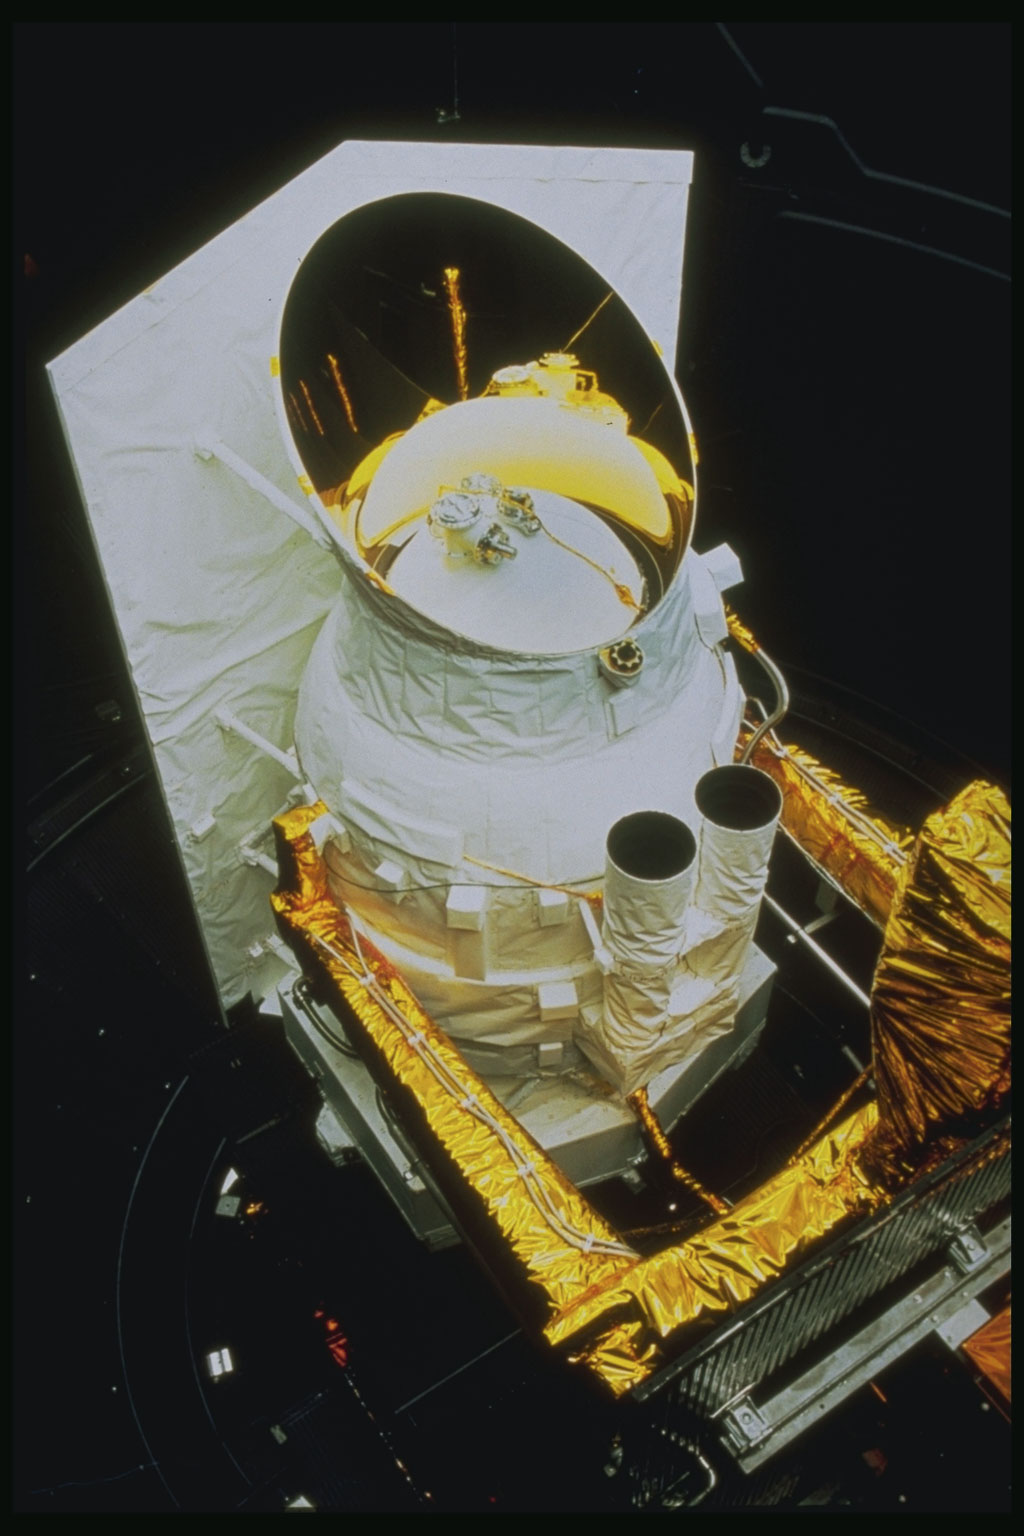
\includegraphics[width=0.30\textwidth]{satellite}
  \end{center}
  \vspace{-20pt}
\end{wrapfigure}
Infrared Space Observatory (ISO) è stato realizzato dall'European Space Agency (ESA) per l'osservazione dell'Universo nella \textbf{banda dell'infrarosso}.
E’stato lanciato il 16 novembre 1995 con un razzo Ariane dal centro spaziale di Kourou, ha cessato la sua attività nell'aprile 1998.
Il satellite è stato realizzato per effettuare il primo censimento dettagliato delle sorgenti di radiazione infrarossa, sia di quelle normalmente invisibili, a causa dell'assorbimento atmosferico, sia delle quasar distanti e delle galassie superluminose. 

\section*{Osservazioni}
\label{osservazioni}

Il satellite alto 5,3 m, largo 3,5 m e con una massa al lancio di 2400 kg, è dotato di apparecchiature per la ricerca di sistemi planetari esterni al sistema solare, ha compiuto studi sui processi relativi alla nascita delle stelle e alla formazione dei pianeti e indagini sia sulle galassie attive con un eventuale buco nero nel loro nucleo, sia sulle galassie in formazione oscurate dalle polveri cosmiche. 

In tre anni, il satellite ha compiuto 26.000 osservazioni delle profondità dell'Universo, individuando fenomeni mai osservati prima come gli \textbf{anelli di Andromeda}, una delle galassie più vicine alla Terra e più studiate. Ha individuato, anche, la sua vera struttura, che da spirale sta assumendo una forma circolare, gli archi gravitazionali attraverso le immagini di galassie in collisione, l'acqua nello spazio e gli anelli di materia organica intorno a giovani stelle.

\section*{Curiosità}
\label{curiosit}

L'ISO, la cui vita operativa è terminata in seguito alla vaporizzazione dell'elio, ha percorso in 24 ore un'orbita di 1000 km. L'orbita allungata ha permesso al satellite di restare per ca. 16 ore al giorno al di fuori della zona di radiazioni che circondano la Terra. Il controllo dalla Terra è avvenuto dalla stazione ESA di Villafranca, in Spagna. Il suo telescopio, puntato per periodi di ca. 10 ore, ha avuto una precisione di alcuni secondi d'arco e una sensibilità all'infrarosso tale da poter rilevare il calore di un cubetto di ghiaccio a 100 km di distanza sullo sfondo astronomico molto più freddo. 

Dalle osservazioni compiute da ISO, un gruppo di astrofisici tedeschi hanno ipotizzato: che due oggetti ritenuti diversi, come i quasar e le radiogalassie, possano essere probabilmente la stessa cosa, che le supposte differenze siano in realtà solo illusioni ottiche causate dal nostro punto di osservazione, la Terra, e che entrambi abbiano al centro un buco nero massivo circondato da una cortina di polvere. 


\end{document}